\thispagestyle{cackithitoannone}
\pagestyle{cackithitoan}
\everymath{\color{cackithi}}
\graphicspath{{../cackithi/pic/}}
\begingroup
\AddToShipoutPicture*{\put(0,616){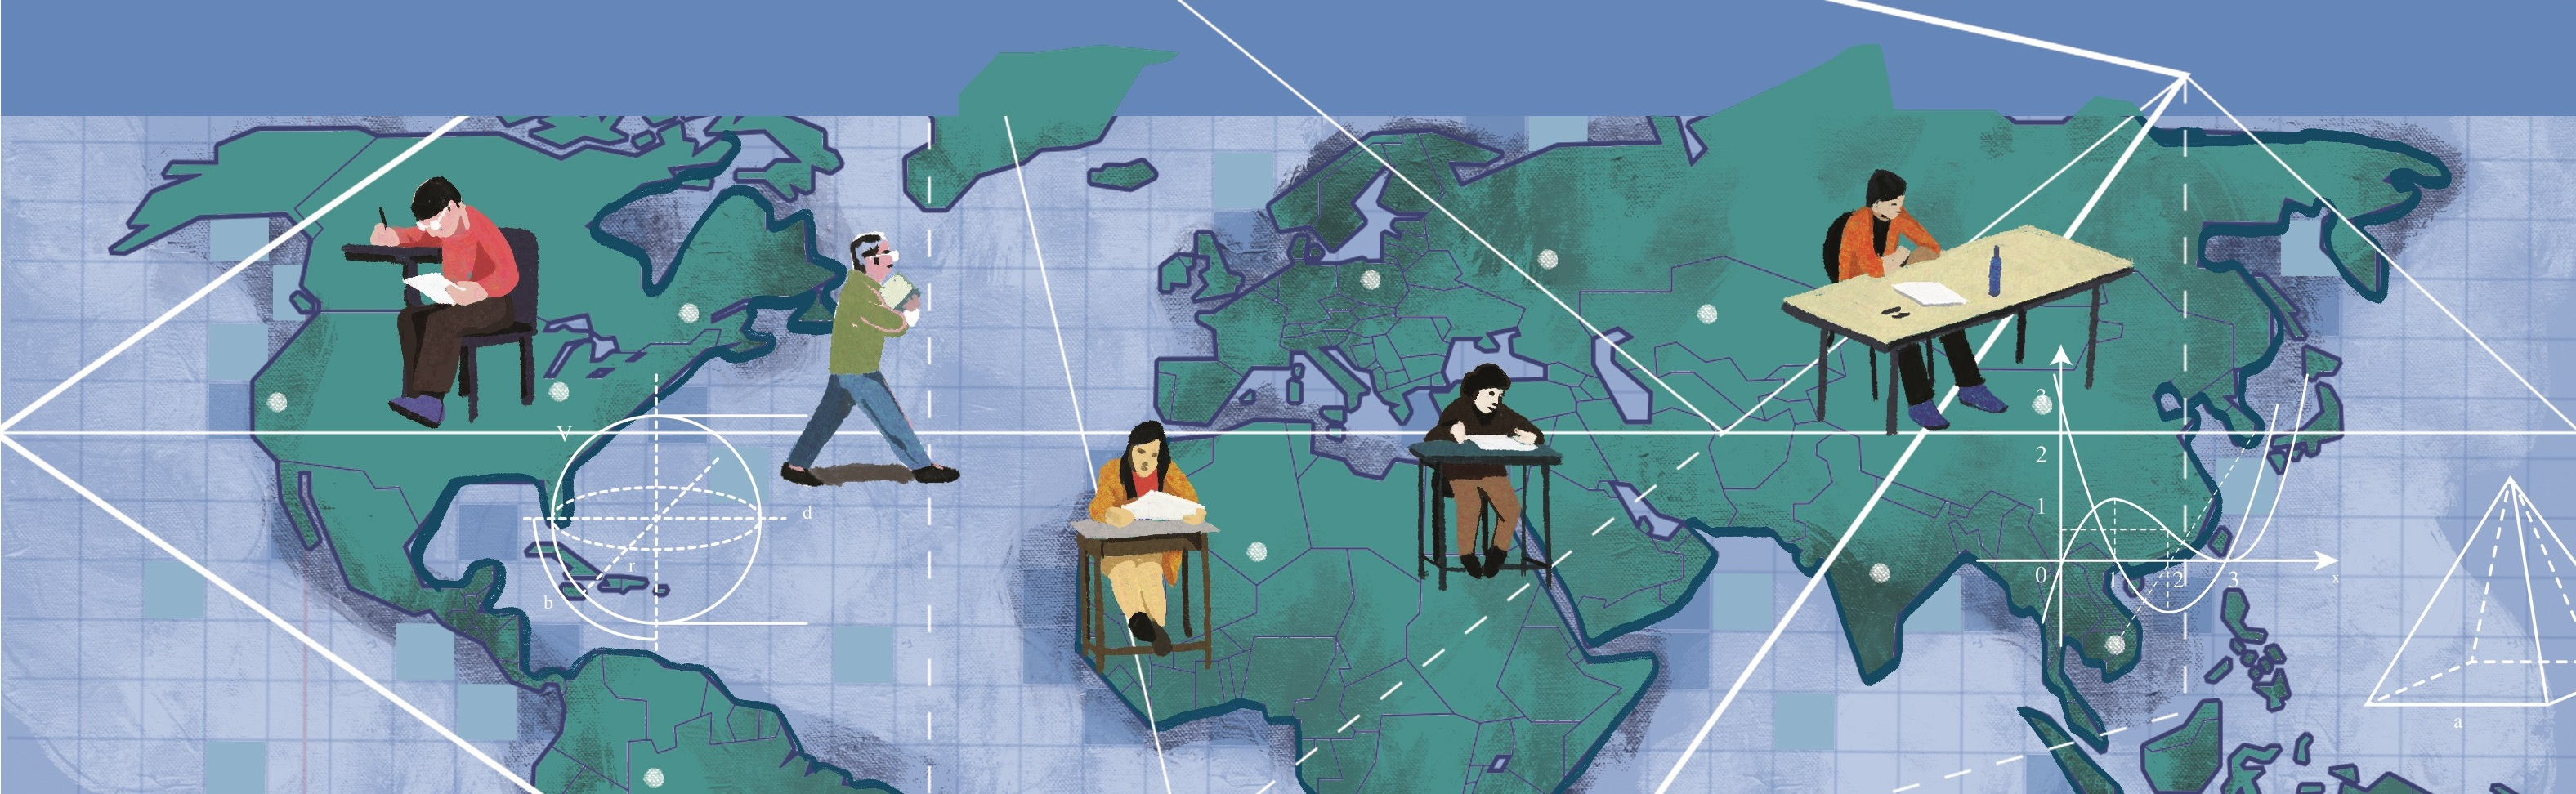
\includegraphics[width=19.3cm]{../bannercackithi}}} 
\AddToShipoutPicture*{\put(150,575){
\includegraphics[scale=1]{../tieude1.pdf}}}
\centering
\endgroup
\vspace*{130pt}

\begin{multicols}{2}
	Trong phần đầu chuyên mục, chúng tôi sẽ trình bày lời giải của các bài toán trong kỳ thi  Olympic Toán học Trẻ của Canada năm học $2022$  đăng trong số báo $11/2022$. 
	\vskip 0.1cm
	{\bf\color{cackithi} OC$\pmb{25.}$} Cho $ABC$ là tam giác nhọn nội tiếp đường tròn $\Gamma.$ Đường thẳng qua $A$ vuông góc với $BC$ cắt $\Gamma$ tại $D,$ và đường thẳng qua $B$ vuông góc với $AC$ cắt $\Gamma$ tại $E.$ Chứng minh rằng nếu $AB = DE$, thì $\angle ACB = 60^{\circ}.$
	\vskip 0.1cm
	\textit{Lời giải.} 
	\begin{figure}[H]
		\vspace*{-5pt}
		\centering
		\captionsetup{labelformat= empty, justification=centering}
		\begin{tikzpicture}[cackithi]
			\draw (0.9004185552987112,2.2669457035324743) -- (1.0180882363816217,2.0904411819081083) -- (1.1945927580059874,2.208110862991019) -- (1.0769230769230769,2.3846153846153846) -- cycle; 
			\draw (-0.4987538820250189,1.8329179606750063) -- (-0.4316718427000252,2.0341640786499875) -- (-0.6329179606750064,2.101246117974981) -- (-0.7,1.9) -- cycle; 
			\draw  (0.5,2.1666666666666665) circle (1.9002923751652299cm);
			\draw  (-1.,1.)-- (2.,1.);
			\draw  (2.,1.)-- (0.,4.);
			\draw  (0.,4.)-- (-1.,1.);
			\draw  (-1.,1.)-- (2.1538461538461533,3.102564102564102);
			\draw  (2.,1.)-- (-1.4,2.1333333333333333);
			\draw  (-1.4,2.1333333333333333)-- (2.1538461538461533,3.102564102564102);
			\draw  (2.1538461538461533,3.102564102564102)-- (0.,4.);
			\draw  (0.,4.)-- (-1.4,2.1333333333333333);
				\draw [fill=white] (-1.,1.) circle (1.5pt);
				\draw (-1.3,0.79) node {$A$};
				\draw [fill=white] (2.,1.) circle (1.5pt);
				\draw (2.3,0.77) node {$B$};
				\draw [fill=white] (0.,4.) circle (1.5pt);
				\draw (0.,4.45) node {$C$};
				\draw [fill=white] (2.1538461538461533,3.102564102564102) circle (1.5pt);
				\draw (2.36,3.49) node {$D$};
				\draw [fill=white] (-1.4,2.1333333333333333) circle (1.5pt);
				\draw (-1.7,2.21) node {$E$};
		\end{tikzpicture}
		\vspace*{-10pt}
	\end{figure}
	Do $ABC$ là tam giác nhọn nên các điểm $D$ và $E$ lần lượt nằm ở bên trong cung nhỏ $BC$ và $AC$ như trong hình vẽ. Như vậy $\angle ECD$ lớn hơn  $\angle ACB$. Từ giả thiết $AB=DE,$ ta có $\angle ECD= 180^\circ - \angle ACB$.  \hfill ($1$)
	\vskip 0.1cm
	Mặt khác ta có
	\begin{align*}
		\angle ECD =\,&\angle ECA + \angle ACB + \angle BCD \\
		= \,&\angle EBA + \angle ACB + \angle BAD \\
		= \,&90^\circ \!\!-\!\! \angle BAC \!\!+\!\! \angle ACB \!\!+\!\! 90^\circ \!\!-\!\! \angle ABC \\
		= \,&(180^\circ \!-\! \angle BAC \!-\! \angle ABC) \!+\! \angle ACB  \\
		= \,&2\angle ACB  \tag{$2$}
	\end{align*}
	Từ ($1$) và ($2$) ta nhận được điều cần chứng minh.
	\vskip 0.1cm
	{\bf\color{cackithi} OC$\pmb{26.}$} Giả sử bạn có vô hạn các hình chữ $T$ (bao gồm bốn hình vuông cạnh
	$1$) như trong hình vẽ, và một bảng ô vuông cỡ $n \times n.$ Bạn được phép đặt một số hình trên bảng (có thể xoay chúng), miễn là không có hai hình nào chồng lên nhau và không có hình nào vượt ra khỏi bảng.
	\vskip 0.1cm
	Với những giá trị nào của $n$ thì bạn có thể phủ toàn bộ bảng?
	\begin{figure}[H]
		\vspace*{-5pt}
		\centering
		\captionsetup{labelformat= empty, justification=centering}
		\begin{tikzpicture}[cackithi,scale=0.88]
			\draw (0,0) grid (3,1);
			\draw (1,-1) grid (2,0);
		\end{tikzpicture}
		\vspace*{-10pt}
	\end{figure}
	\textit{Lời giải.} Trước tiên ta nhận thấy mỗi hình chữ $T$ gồm $4$ ô, do đó nếu phủ kín được bảng thì diện tích của bảng phải chia hết cho $4$, tức là $n$ chẵn.
	\vskip 0.1cm
	Với $n$ chia hết cho $4$ ta có thể chia bảng thành các bảng con cỡ $4\times 4$ và phủ kín mỗi bảng con bằng $4$ hình chữ $T$ như sau:
	\begin{figure}[H]
		\vspace*{-5pt}
		\centering
		\captionsetup{labelformat= empty, justification=centering}
		\begin{tikzpicture}[cackithi,scale=0.88]
			\filldraw[duongvaotoanhoc] (0,0) rectangle (3,1);
			\filldraw[gocco] (3,0) rectangle (4,3);
			\filldraw[timhieukhoahoc] (4,3) rectangle (1,4);
			\filldraw[toanhocdoisong] (0,1) rectangle (1,4);
			\filldraw[duongvaotoanhoc] (1,1) rectangle (2,2);
			\filldraw[gocco] (2,1) rectangle (3,2);
			\filldraw[timhieukhoahoc] (2,2) rectangle (3,3);
			\filldraw[toanhocdoisong] (1,2) rectangle (2,3);
			\draw (0,0) grid (4,4);
		\end{tikzpicture}
		\vspace*{-10pt}
	\end{figure}
	Với $n=4k+2,$ ta tô màu đen, trắng các ô trong bảng như bàn cờ vua. Để lát kín bảng cần tất cả $\dfrac{n^2}{4}=(2k+1)^2$ hình chữ $T$. Như vậy có một số lẻ hình chữ $T$ và mỗi hình phủ $1$ hoặc $3$ ô đen, tức là tổng số ô đen phải là lẻ. Nhưng thực tế có  $\dfrac{n^2}{2}=2(2k+1)^2$ ô đen. Do đó trường hợp này không thể phủ kín bảng như yêu cầu. 
	\begin{figure}[H]
		\vspace*{-5pt}
		\centering
		\captionsetup{labelformat= empty, justification=centering}
		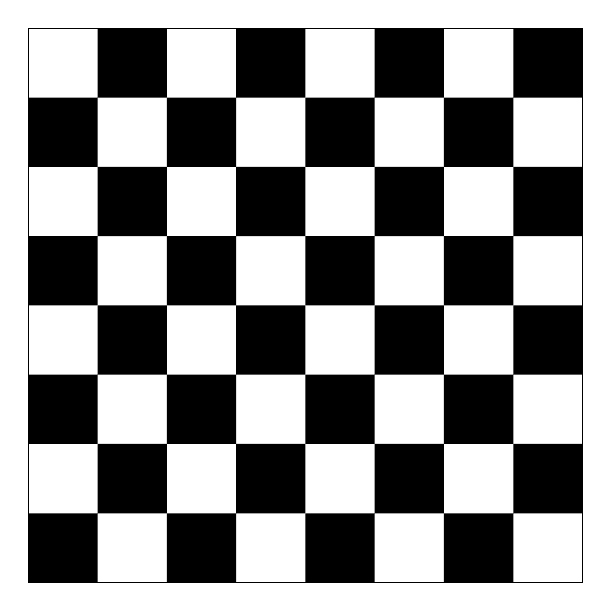
\begin{tikzpicture}[scale=0.88]
			\draw (0,0) rectangle (8,8);
			\foreach \y in {0,2,...,6}{
				\foreach \x in {0,2,...,6}{
					\fill (\x,\y) rectangle (1+\x,1+\y) rectangle (2+\x,2+\y);}}
		\end{tikzpicture}
		\vspace*{-5pt}
	\end{figure}
	Tóm lại ta phủ kín được bảng bằng các hình chữ $T$ khi và chỉ khi $n$ chia hết cho $4$.
	\vskip 0.1cm
	{\bf\color{cackithi} OC$\pmb{27.}$} Giả sử rằng các số thực $a$ và $b$ thỏa mãn
	\begin{align*}
		ab+ \sqrt{ab+1} +\sqrt{a^2+b}\ \sqrt{b^2+a}=0.
	\end{align*}
	Tìm giá trị của biểu thức
	\begin{align*}
		S=a\sqrt{b^2+a} + b\sqrt{a^2+b}.
	\end{align*}
	\textit{Lời giải.} Từ đẳng thức trong bài, chuyển vế và bình phương hai vế ta có
	\begin{align*}
		& \ ab+ \sqrt{a^2+b} \sqrt{b^2+a} = \sqrt{ab+1} \\
		\Rightarrow\  &	a^2b^2 + 2ab\sqrt{a^2+b} \sqrt{b^2+a} \\
		&+ (a^2+b)(b^2+a) = ab+1\\
		\Leftrightarrow\  &	(a^2b^2+a^3) + 2ab\sqrt{a^2+b} \sqrt{b^2+a} \\
		&+ (b^3+a^2b^2) = 1\\
		\Leftrightarrow\ 	& (a\sqrt{b^2+a} + b\sqrt{a^2+b})^2 = 1.
	\end{align*}
	Ta nhận được $S=\pm 1.$ Ta sẽ chứng minh $S$ luôn dương. Thực vậy, từ giả thiết ta có
	\begin{align*}
		ab= -\sqrt{ab+1} -\sqrt{a^2+b} \sqrt{b^2+a} <0.
	\end{align*}
	Không mất tổng quát, ta có thể giả sử \linebreak $a>0>b.$ Khi đó, do $a>\sqrt{a^2+b},$ ta có
	\begin{align*}
		S= a( \sqrt{b^2+a} +b)- b(a- \sqrt{a^2+b})>0.
	\end{align*} 
	Do đó  $S=1$.
	\vskip 0.1cm
	Trong phần cuối của chuyên mục kỳ này, chúng tôi sẽ giới thiệu với bạn đọc ba bài toán trong kỳ thi Olympic Toán học trẻ khối Pháp ngữ năm $2022$. Các bài toán này phù hợp với trình độ học sinh năm cuối cấp Trung học cơ sở.
	\vskip 0.1cm
	{\bf\color{cackithi} OC$\pmb{34.}$} Tìm tất cả các số nguyên dương $n$ sao cho $ \lfloor \sqrt{n}\rfloor $ là ước của $n.$ 
	\vskip 0.1cm
	\textit{Chú ý}: $ \lfloor x \rfloor $ ký hiệu phần nguyên của một số thực $x,$ được định nghĩa là số nguyên lớn nhất nhỏ hơn hoặc bằng $x.$ Ví dụ: $ \lfloor 1.4 \rfloor =1$, $ \lfloor 2 \rfloor=2,$ và  $ \lfloor 2.9 \rfloor= 2.$  
	\vskip 0.1cm
	{\bf\color{cackithi} OC$\pmb{35.}$} Cho một bảng ô vuông cỡ $n \times n$ với $n\ge 1$. Aya muốn tô màu  $k$ ô của bảng  sao cho chỉ có duy nhất một cách để đặt  $n$ đồng xu trên các ô vuông được tô màu sao cho không có hai đồng xu nào nằm trên cùng một hàng hoặc cột. Hỏi giá trị tối đa có thể của $k$  là bao nhiêu?
	\vskip 0.1cm
	{\bf\color{cackithi} OC$\pmb{36.}$} Cho tam giác $ABC$ và $D$ là giao điểm của đường phân giác của góc $\angle BAC$ và đường trung trực của cạnh $AC$. Đường thẳng  đi qua $B$ và song song với $AC$, cắt đường thẳng $AD$ tại $X$. Đường thẳng đi qua $B$ và song song với $CX$, cắt đường thẳng $AC$ tại $Y$. Đường tròn ngoại tiếp tam giác $ABY$ cắt đường thẳng $BX$ tại $E.$ Chứng minh rằng ba điểm $C$ , $D$ và $E$ thẳng hàng.
\end{multicols}